% =====================================================================
% Clase -- Física 9° -- Trimestre I -- Semana 05
% Sesión 004 (lun 28 sep., 10:10, 50 min)
% Tema: Describir el movimiento
% Subtema: Marco de referencia, posición y trayectoria
% Hilo conductor del trimestre I: «De Aristóteles a Galileo: aprender a describir el movimiento»
% Tema 2 de la guía: Describir el movimiento (tema:describir)
% Material del docente (no se entrega a los estudiantes).
% =====================================================================
\documentclass[11pt]{article}
\makeatletter\def\input@path{{../../../../../plantillas/estilo/}}\makeatother
\usepackage{mmcantillo}
\guiadelestudiante{../../guia-didactica/guia-periodo-I-movimiento}

\tipodocumento{Clase}
\asignatura{Física}
\titulo{Semana 5: decir desde dónde se mira}
\grado{9°}
\periodo{I}

% DBA: naturales grado 9 · DBA 1 — Comprende que el movimiento de un cuerpo, en un marco de
% referencia inercial dado, se puede describir con gráficos y predecir por medio de
% expresiones matemáticas. Evidencia de esta sesión: la primera del DBA — establecer un marco
% de referencia y describir en él la posición, la trayectoria y el desplazamiento de un
% cuerpo, que es el requisito para las gráficas y las expresiones de las sesiones siguientes.

\begin{document}

\encabezado*

\begin{center}
{\renewcommand{\arraystretch}{1.3}
\begin{tabularx}{\linewidth}{@{}l l l X l@{}}
  \toprule
  \textbf{Sesión} & \textbf{Fecha} & \textbf{Min} & \textbf{Subtema} & \textbf{Entregables}\\
  \midrule
  004 & lun 28 sep., 10:10 & 50 & Marco de referencia, posición y trayectoria
      & Se deja tarea (5 pts)\\
  \bottomrule
\end{tabularx}}
\end{center}

Las dos semanas pasadas cerramos con una idea: los griegos querían \emph{explicar} por qué se
mueven las cosas, y Galileo empezó por \emph{describir} cómo se mueven. Hoy damos el primer
paso de esa descripción, y es más raro de lo que parece: antes de medir nada hay que decir
desde dónde se mide. Sin eso, la pregunta «¿este cuerpo se está moviendo?» no tiene respuesta.
Referencia: \refguia{tema:describir}.

% ---------------------------------------------------------------------
\seccion{Sesión 004 — lunes 28 de septiembre · 10:10 · 50 min}

\textbf{Objetivo.} Establecer un marco de referencia (origen y sentido positivo), escribir la
posición de un cuerpo en él, y distinguir trayectoria, distancia recorrida y desplazamiento.

\textbf{Materiales.} Cinta métrica o metro; tiza para marcar el piso del salón o el corredor;
la guía.

\begin{center}
{\renewcommand{\arraystretch}{1.3}
\begin{tabularx}{\linewidth}{@{}l l X@{}}
  \toprule
  \textbf{Momento} & \textbf{Min} & \textbf{Actividad}\\
  \midrule
  Enganche & 0--8 & Pregunta al salón: «¿Tú te estás moviendo ahora mismo?» Se recogen dos o
    tres respuestas. Después: respecto de la silla, no; respecto del Sol, a más de
    \qty{100000}{km/h}. Las dos respuestas son correctas. \textbf{Moverse no es una propiedad
    del cuerpo: es una relación entre el cuerpo y un marco de referencia.} Esta frase queda
    escrita en el tablero toda la clase.\\
  El eje en el piso & 8--22 & Con tiza se marca un eje en el piso del salón: un origen (la
    puerta) y el sentido positivo hacia el tablero, con marcas cada metro. Un estudiante
    camina y los demás anotan su posición $x$ en cada parada. Se repite \textbf{cambiando el
    origen} a la mitad del salón: los números cambian, pero los cambios de posición no. Ese
    es el descubrimiento de la sesión.\\
  Tres palabras & 22--36 & Definir con lo que acaba de pasar en el piso:
    \textbf{trayectoria} (el camino recorrido), \textbf{distancia recorrida} (su longitud,
    siempre positiva) y \textbf{desplazamiento} $\Delta x = x_f - x_i$ (el cambio de posición,
    con signo). Ejemplo de la guía: caminar \qty{70}{m} al oriente y \qty{30}{m} al occidente
    da \qty{100}{m} de distancia y \qty{+40}{m} de desplazamiento.\\
  La ida y vuelta & 36--45 & El caso que lo aclara todo: quien sale de su casa, da la vuelta a
    la manzana y regresa. Distancia recorrida: todo el perímetro. Desplazamiento: cero. «El
    odómetro de la bicicleta suma; el desplazamiento se fija solo en dónde arrancó y dónde
    terminó.»\\
  Cierre & 45--50 & Se deja la tarea (5 puntos). Anuncio: con la posición y el tiempo ya se
    puede hacer lo que hizo Oresme — dibujar el movimiento — y eso es la próxima sesión.\\
  \bottomrule
\end{tabularx}}
\end{center}

\textbf{Figura para el tablero: el mismo movimiento, dos orígenes.}

\begin{center}
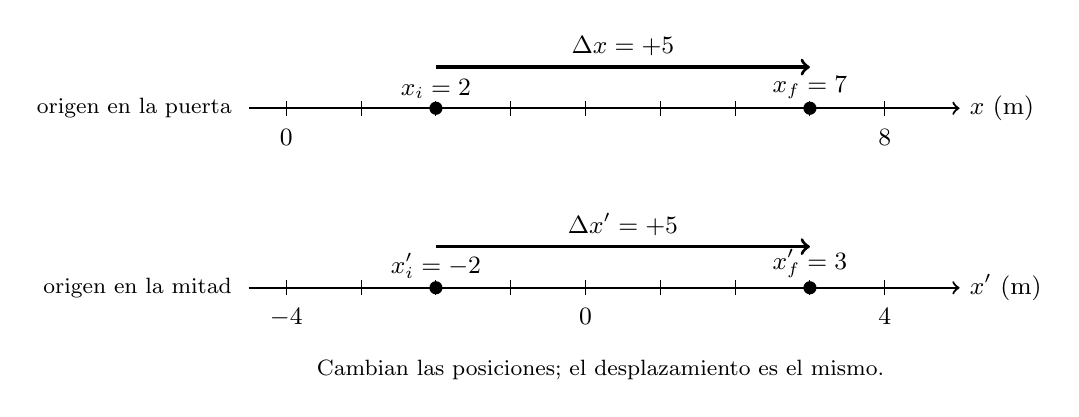
\begin{tikzpicture}[scale=0.95, every node/.style={font=\small}]
  % eje 1
  \draw[->, thick] (-0.5,0) -- (9,0) node[right] {$x$ (m)};
  \foreach \x in {0,1,...,8} \draw (\x,-0.1) -- (\x,0.1);
  \node[below] at (0,-0.15) {$0$};
  \node[below] at (8,-0.15) {$8$};
  \fill (2,0) circle (2.5pt) node[above] {$x_i = 2$};
  \fill (7,0) circle (2.5pt) node[above] {$x_f = 7$};
  \draw[->, very thick] (2,0.55) -- (7,0.55) node[midway, above] {$\Delta x = +5$};
  \node[left, font=\footnotesize] at (-0.6,0) {origen en la puerta};
  % eje 2
  \begin{scope}[yshift=-2.4cm]
    \draw[->, thick] (-0.5,0) -- (9,0) node[right] {$x'$ (m)};
    \foreach \x in {0,1,...,8} \draw (\x,-0.1) -- (\x,0.1);
    \node[below] at (0,-0.15) {$-4$};
    \node[below] at (4,-0.15) {$0$};
    \node[below] at (8,-0.15) {$4$};
    \fill (2,0) circle (2.5pt) node[above] {$x'_i = -2$};
    \fill (7,0) circle (2.5pt) node[above] {$x'_f = 3$};
    \draw[->, very thick] (2,0.55) -- (7,0.55) node[midway, above] {$\Delta x' = +5$};
    \node[left, font=\footnotesize] at (-0.6,0) {origen en la mitad};
  \end{scope}
  \node[font=\footnotesize] at (4.2,-3.5)
    {Cambian las posiciones; el desplazamiento es el mismo.};
\end{tikzpicture}
\end{center}

\begin{nota}
\textbf{Dónde suele trabarse.} En creer que el desplazamiento negativo significa «menos
camino» o «se equivocó». El signo no mide cantidad, indica sentido: $\Delta x = \qty{-600}{m}$
es tanto camino como $\qty{+600}{m}$, pero hacia el otro lado. Conviene decirlo con las manos,
señalando los dos sentidos del eje del piso.
\end{nota}

\begin{nota}
\textbf{El experimento del piso.} Vale la pena no saltárselo aunque tome tiempo: la idea de
que los números cambian con el origen pero el desplazamiento no es abstracta si se escribe en
el tablero, y obvia si se camina. Si el salón es estrecho, sirve el corredor de afuera.
\end{nota}

\begin{nota}
\textbf{Conexión con matemáticas.} La resta $x_f - x_i$ es la misma que usan en Geometría para
la distancia entre dos puntos de un eje. Si alguien lo nota, vale la pena celebrarlo: no son
dos fórmulas, es una sola idea en dos asignaturas.
\end{nota}

\end{document}
